\documentclass[runningheads]{llncs}
\usepackage{graphicx}
\usepackage[width=122mm,left=12mm,paperwidth=146mm,height=193mm,top=12mm,paperheight=217mm]{geometry}
\usepackage{amsmath,amssymb} % define this before the line numbering.
%\usepackage{ruler}
\usepackage{color}

%\documentclass{llncs}
%\usepackage{graphicx}
%\usepackage{geometry}
%\geometry{margin=2cm}
%\usepackage{amsmath}

\usepackage{pgfplots}
\usepackage{filecontents}
\usepackage[caption=false]{subfig}
\usepackage{listings}
\lstset{
basicstyle=\small\ttfamily,
columns=flexible,
breaklines=true
}

\begin{document}
\title{Dissecting Neural Style Transfer}
\author{Xi Du}
\institute{Australian National University, Australia\\
\email{u6559090@anu.edu.au}}
\maketitle 
\begin{abstract}
\cite{method}

\keywords{Neural network, Deep learning, 
Small data, Interpretability, Network pruning, Network reduction.}
\end{abstract}

\section{Introduction}

\section{Literature Review}

\section{Method}

\subsection{Deep Neural Network}

For the purpose of implementing and even extending neural style transfer algorithms,
it is not necessary to understand how a neural network is trained, because
we can use pretrained model for example vgg19 \cite{vgg19}.

It is necessary to point out that a deep neural network that neural style transfer
is concerend about
is just a sequence of functions
$F_1,F_2,F_3,...$
whose inputs and outputs are all multi-dimensional arrays, as illustrated in Figure \ref{f1f2f3}.
\begin{figure}
\center
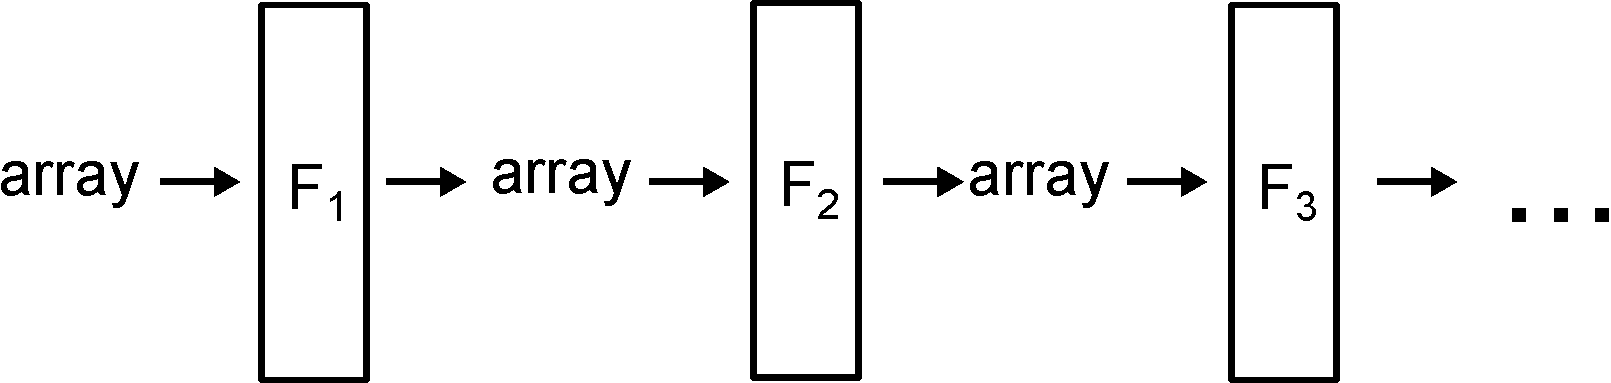
\includegraphics[width=0.6\textwidth]{f1f2f3.pdf}
\caption{A deep neural network \label{f1f2f3}}
\end{figure}
Because the arrays have usually more than two numbers of dimensions
they are not really matrices.
The arrays are called tensors (as in TensorFlow or torch.Tensor in PyTorch) 
but actual tensor algebra in a mathematical sense is rarely relevant.
The functions need to be differentiable, which is handled automatically by modern 
deep learning frameworks.
Other than that we can treat the functions as blackboxes because we are 
not concerned of training the model.

For the vgg19 model that most neural style transfer implementations available are based on,
The inputs and outpus of each layer are all arrays with 4 dimensions.
The word ``dimension'' here may mean something slightly different from what ``dimension'' means in
for example ``$3$-dimension vector''. 
Some people call the number of dimensions ``rank'' which would then raise another confusion with the rank of matrices.

The 1st dimension is the ``batch'' dimension, which means that you can put several images through the
series of functions.
In neural style transfer implementations it is usually just one image each time.
So the 1st dimension is always 1, even between the $F$ functions, throughout this work.

The 2nd dimension is the ``feature'' dimension. For a raw RGB image, it is 3.
Intermediate values between, for example, $F_3$ and $F_4$, usually 
have a size much larger than 3, such as 64 or 128



\subsection{Vanilla neural style transfer}

\subsection{Implementation of Neural Network}
Since we are not training the neural network, 
the model is just a sequence of functions on arrays.

\subsubsection{Testing Phase}

\subsection{Data Set}

\subsubsection {Format and Preparation}

\subsubsection {(Not Really) Time-Series}

\subsubsection {Rationale}

\subsection{Hyperparameters and Experiments}

For the vanilla style-transfer algorithm, there were a few hyper-parameters that 
affected the result.
\begin{itemize}
\item Number of iterations in the optimization. 
We did not have to expriment with different numbers of iterations though.
It was more sensible to run the algorithm for more-than-enough iterations and store the intermediate results.
\item Weights of style loss $k_S$ and content loss $k_C$ in the optimisation target. 
Although these appeared to be two parameters,
actually only their ratio $k_S/k_C$ mattered.
We simply fixed $k_C=1$ and varied $k_S$.
\item Choice of initial values. Some sensible choices were:
\begin{itemize}
\item White noise.
\item White.
\item Black.
\item The model mean.
\item The content image.
\item The style image.
\item The average of the content image and the style image.
\end{itemize}
\end{itemize}

%\subsubsection{Activation Function}

\subsubsection{Learning Rate}

\subsubsection{Hidden Layer Size}

\subsection{Evaluating Prediction}

\subsubsection{Binarisation and Choice of Loss}

\subsubsection{Amount of Network Reduction}

\subsubsection{Mechanism} 

\subsubsection{Execution}

The program was developed under and are compatible with:
\begin{itemize}
\item Python 3.6
\item PyTorch 1.0.1.post2
\item CentOS 7 x86\_64
\end{itemize}
To run the code, execute shell commands like
\begin{verbatim}
python36 0.py 5000
\end{verbatim}
where 5000 is the number of desired training cycles to reach.
The different hyperparameters will be automatically covered.
The program automatically picks up stored models.
To start fresh, clear the stored models and outputs by
\begin{verbatim}
rm out/*/*.*
\end{verbatim}
but do not remove the directories.


\section{Results and Discussion}

\section{Conclusion and Future Work}

\begin{thebibliography}{8}
\bibitem{nst}
Gatys, L., Ecker, A., \& Bethge, M. (2016). A neural algorithm of artistic style. Journal of Vision, 16(12), 326. doi:10.1167/16.12.326
\bibitem{method}
Gedeon, T.D. and Harris, D. (1991) "Network Reduction Techniques," Proceedings International Conference on Neural Networks Methodologies and Applications, AMSE, San Diego, vol. 1: 119-126. 
\bibitem{prune0}
Penington, Jocelyn \& Dow, R.J.F.. (1988). Neural net pruning—Why and how. Proceedings of the IEEE Conference on Neural Networks. 1. 325 - 333 vol.1. 10.1109/ICNN.1988.23864. 
\bibitem{interp}
Doshi-Velez, F., \& Kim, B. (2017). Towards A Rigorous Science of Interpretable Machine Learning.
\bibitem{example_prune}
Han, S., Mao, H., \& Dally, W.J. (2016). Deep Compression: Compressing Deep Neural Network with Pruning, Trained Quantization and Huffman Coding. CoRR, abs/1510.00149.
\bibitem{example_simplification}
Sun, X., Ren, X., Ma, S., Wei, B., Li, W., \& Wang, H. (2018). Training Simplification and Model Simplification for Deep Learning: A Minimal Effort Back Propagation Method. CoRR, abs/1711.06528.
\bibitem{example_compression}
Cheng, Yu \& Wang, Duo \& Zhou, Pan \& Zhang, Tao. (2017). A Survey of Model Compression and Acceleration for Deep Neural Networks. 
\bibitem{pytorch}
Paszke, A., Gross, S., Chintala, S., Chanan, G., Yang, E., DeVito, Z., Lin, Z., Desmaison, A., Antiga, L., \& Lerer, A. (2017). Automatic differentiation in PyTorch.
\end{thebibliography}
\end{document}

